% SSC 2027 full paper draft (Springer LNCS).
% Every number in Sections 5-6 comes from raw_materials/experimental_log.md.
\documentclass[runningheads]{llncs}

\usepackage[utf8]{inputenc}
\usepackage{graphicx}
\usepackage{amsmath,amssymb}
\usepackage{booktabs}
\usepackage{array}
\newcolumntype{L}[1]{>{\raggedright\arraybackslash}p{#1}}
\usepackage{xcolor}
\usepackage{hyperref}
\renewcommand\UrlFont{\color{blue}\rmfamily}
\emergencystretch=1.5em

% Marker for content that waits for a decision of the authors.
\newcommand{\pending}[1]{\textcolor{red}{[\textsc{pending}: #1]}}

\begin{document}

\title{Incentives or Wording? Auditing LLM Decision Rules in Public Goods Games}
\titlerunning{Incentives or Wording? Auditing LLM Decision Rules}

\author{Jos\'e Pinto-Mu\~noz \and Sof\'ia Herrera-Henr\'iquez}
\authorrunning{J. Pinto-Mu\~noz and S. Herrera-Henr\'iquez}
\institute{Universidad T\'ecnica Federico Santa Mar\'ia, Chile\\ \email{jose.pintom@usm.cl, sofia.herrerah@usm.cl}}

\maketitle

\begin{abstract}
Large language models (LLMs) are increasingly used as decision rules for agents in social simulations, yet it is unclear whether their choices follow the incentives encoded in a model or the wording used to describe it. We audit six current fast-tier LLMs in a linear public goods game, in two studies with plans fixed in advance. In one-shot decisions we vary the marginal per capita return inside the social dilemma and in two controls where self-interest and collective welfare coincide, under payoff-equivalent paraphrases and three framings. Without explicit reasoning, rewording the same game explains 3 to 21 times more variance in contributions than the incentive in five models, and no model chooses the dominant action in both controls. With reasoning switched on, three of five models contribute nothing under every wording inside the dilemma, so paraphrase no longer matters there. Where contributing is the dominant action, two models still range over 70 and 82 percentage points across wordings. In ten-round games with feedback, the gap between a ``Teamwork'' label and the named game is still present in the last round in three of six models and vanishes in the others. One model answered an identical prompt with full contribution in 91\% of decisions in one batch and in 10\% an hour later. In this audit, cooperation is set largely by wording and reasoning mode and only weakly by the modelled incentives. Protocol, prompts and data are public.

\keywords{Large language models \and Agent-based modelling \and Public goods game \and Validation \and Prompt sensitivity}
\end{abstract}

\section{Introduction}

Large language models (LLMs) enter agent-based modelling mainly as the decision rule of the agent. In a recent review for this community, 20 of 22 coded studies used the LLM at the implementation stage, as the engine that decides or communicates on the agent's behalf~\cite{vanhee2026llmabm}.

It is less clear that the action can be trusted. A critical review of generative agent-based models finds that 15 of 35 studies rely solely on subjective assessments for validation and that most draw conclusions from a single run~\cite{larooij2026validation}. Edmonds argues that neither the plausibility of LLM output nor clever prompting is sufficient, and that one needs to check that the system behaves reliably for the modelling purpose~\cite{edmonds2026when}.

We carry out such a check for one well-understood situation and ask two things of an LLM used as a decision rule. When the modeller changes a payoff parameter, does the action change in a direction that theory or evidence predicts? When the modeller rewrites the description without changing the payoffs, does the action stay the same? If wording moves behaviour more than incentives do, the simulation reports the modeller's phrasing instead of the modelled mechanism.

The linear public goods game suits this audit because it offers independent references. In the Nash equilibrium of the one-shot game nobody contributes. In laboratory experiments people contribute between 40 and 60 percent of their endowment at first and contribute more when the return on contributions is higher~\cite{ledyard1995public,zelmer2003meta,isaac1988group}. A third reference is Adam Smith, whose invisible hand is often said to fail in this game. Smith did not expect it to work there. He assigned to the sovereign those public works which, ``though they may be in the highest degree advantageous to a great society, are, however, of such a nature that the profit could never repay the expence to any individual or small number of individuals''~\cite[V.i.c]{smith1776wealth}. On voluntary provision Smith and Nash agree. The contrasting prediction comes from Smith's other book, which opens by stating that however selfish man may be supposed, ``there are evidently some principles in his nature, which interest him in the fortune of others''~\cite[I.i.1]{smith1759moral}, and which behavioural economists read as anticipating other-regarding behaviour in laboratory games~\cite{ashraf2005smith}. Human subjects fall between the two. We ask where LLM agents fall, and what decides it.

We contribute an audit protocol for LLM decision rules in the linear public goods game, built on payoff-equivalent prompt variants and on control conditions outside the social dilemma. With it we obtain incentive-response curves for six current models, a decomposition of contribution variance into incentive, paraphrase and framing components, and evidence on what reasoning and repeated interaction change. The answer matters for simulations that inform public decisions, where a good that appears to provide itself makes the institutions Smith thought necessary look redundant. We release code, prompts and data.

\section{Related Work}

\paragraph{LLM agents in public goods games.}
The closest study is $\gamma$-Bench~\cite{huang2025gama}, whose public goods game has ten agents of one model playing 20 rounds at $m=0.2$. For GPT-3.5 the authors vary the multiplier over five values, test five prompt templates with one run each, never above the group size, and report that the model contributes similarly even when the return is zero. Li and Shirado~\cite{li2025spontaneous} use four players, one payoff configuration and a binary action, and find that reasoning variants cooperate far less. Sreedhar et al.~\cite{sreedhar2025simulating} show with one model that calling the task ``Teamwork'' instead of ``Taxation'' moves contributions from above 60 to below 40 percent, and list their fixed multiplier as a limitation. Pal et al.~\cite{pal2026llm} vary payoffs and continuation probability in the repeated prisoner's dilemma under a neutral description and assess consistency qualitatively. None of these designs varies the return inside and outside the dilemma under several payoff-equivalent wordings.

\paragraph{Framing and prompt sensitivity.}
Lor\`e and Heydari~\cite{lore2024strategic} cross four two-player games with five narrative contexts and apportion the variation in choices between game structure and context, and Ko\v{r}\'inek and \v{S}tekerov\'a~\cite{korinek2026words} report that positively worded and survival-themed prompts raise cooperation in the iterated prisoner's dilemma with constant payoffs. Such manipulations change the content of the scenario. We are not aware of a study that separates them from content-preserving rewording in one factorial design. For human subjects, presenting the same payoffs as a positive or a negative externality changes contributions~\cite{andreoni1995warm}. We reuse that manipulation.

\paragraph{Validation of generative agent-based models.}
Larooij and T\"ornberg~\cite{larooij2026validation} require that validation match the purpose of the model, be grounded in external evidence, and be robust across runs, and warn that apparent emergence may reproduce phenomena described in the training data. Prompt design can itself predetermine outcomes that are later reported as emergent~\cite{liwu2025letitgo}, and stronger reasoning can move behaviour towards the theoretical solution and away from human data~\cite{kitadai2025reasoning}.

\section{Model}

A group of $N$ agents plays once. Each agent $i$ receives an endowment $E$ and chooses a contribution $c_i \in \{0,1,\dots,E\}$ to a shared account, which is multiplied by $r$ and divided equally:
\begin{equation}
u_i(c_i, c_{-i}) = E - c_i + \frac{r}{N}\sum_{j=1}^{N} c_j .
\label{eq:payoff}
\end{equation}
The marginal per capita return is $m = r/N$ and total welfare is $W = NE + (r-1)\sum_i c_i$. The value of $r$ defines three ranges. If $1<r<N$, each point contributed returns $m<1$ to the contributor and $r>1$ to the group, so contributing nothing is a dominant strategy while contributing everything maximises welfare. This is the social dilemma~\cite{ledyard1995public}. If $r<1$, contributing nothing is both dominant and welfare-maximising. If $r>N$, contributing everything is both dominant and welfare-maximising.

We use the last two ranges as controls. Self-interest and collective welfare point the same way there, so an agent that applies the payoff rule should choose the same action whatever its disposition. A positive contribution when $r<1$, or a partial one when $r>N$, cannot be read as cooperation. The controls also guard against recitation, because the textbook answer to a public goods game is wrong when $r>N$.

In the repeated game the same group plays $T$ rounds with a known horizon. After each round an agent learns the mean contribution of the others and its own payoff. Zero contribution need not be the only equilibrium of a repeated game, so the one-shot equilibrium is only a static reference there.

\paragraph{ODD summary~\cite{grimm2020odd}.}
\emph{Purpose.} The model audits decision rules by measuring how LLM agents respond to a payoff parameter, to the wording of the task and to feedback from other agents. It is not meant to predict human behaviour or to evaluate policy. \emph{Entities.} Agents have a model identifier, a reasoning setting and a prompt variant, and the environment holds $N$, $E$, $r$ and $T$. \emph{Process.} In each round every agent receives the task description, with its own history in the repeated game, and returns one action, which the environment validates before computing payoffs with Eq.~\eqref{eq:payoff}. \emph{Design concepts.} Agents interact only through the shared account and keep no memory beyond the history placed in the prompt. The full description is in the repository. In the scale of Zhao et al.~\cite{zhao2026mechanism} this is a level-1 model, a reproducible phenomenal description from which we draw no counterfactual conclusions.

\section{Experimental Design}
\label{sec:design}

\paragraph{Game and incentives.} $N=4$ and $E=20$, as in a standard human design~\cite{fischbacher2010social}. Inside the dilemma $m\in\{0.3, 0.4, 0.5, 0.75\}$, values used in human experiments~\cite{isaac1988group,fischbacher2010social}. The controls are $m=0.2$ ($r<1$) and $m=1.25$ ($r>N$).

\paragraph{Prompt variants.} All eight variants state the same payoff rule, and an automated test confirms that they imply identical payoffs. The baseline P0 follows the neutral style of Pal et al.~\cite{pal2026llm}. It does not name the game and avoids words such as ``public'', ``cooperate'', ``contribute'', ``group'' and ``team''. Three \emph{paraphrases} carry the same information. P1 reorders the sentences and uses another unit. P2 states what each participant receives per unit placed, $m$, instead of the multiplier, also in another unit. P4 uses an itemised layout. P3 adds two worked examples, for nobody and for everybody placing the full endowment. Three \emph{framings} change the scenario. F1 starts with the endowment in the shared account and asks how much to withdraw~\cite{andreoni1995warm}. F2 calls the task ``Teamwork''~\cite{sreedhar2025simulating}. F3 states that it is a public goods game and uses its usual vocabulary.

\paragraph{Models.} {\sloppy Six models of the fast, low-cost tier were accessed through one inference provider (OpenCode Go) on 17 November 2026. They were \texttt{gpt-5.6-luna}, \texttt{claude-haiku-5-5}, \texttt{qwen3.8-flash}, \texttt{glm-5.3-flash}, \texttt{deepseek-v4.1-flash} (snapshot 1017) and \texttt{hy3}, of which the last three are released with open weights. Temperature was 1.0. All six were run with reasoning disabled. Five were also run with reasoning enabled at high effort, because the provider's interface did not enable reasoning for \texttt{gpt-5.6-luna}.\par}

\paragraph{Study 1: one-shot decisions.} With reasoning off the design is fully crossed, with 6 models $\times$ 6 values of $m$ $\times$ 8 variants $\times$ 50 decisions, or 14,400 decisions. The five models with reasoning add 1,500 decisions on the baseline prompt. Two payoff-calculation questions about the baseline rule were asked in separate calls, 2,040 in total. Each decision is one independent call in shuffled order. An output without a valid action was recorded as invalid and the cell was queried once more. All 17,940 planned cells were completed.

The analysis plan was fixed after a pilot of 576 calls that is excluded from the analysis.\footnote{Both plans were written before the corresponding runs, with hashes of prompts, code and configurations, and neither was posted to a registry such as OSF. The plan of Study~1 was made public after its run and that of Study~2 before its run. Both are in the repository.} Two choices followed the pilot. Hypothesis H6 was added, and the variant with worked examples, first planned as a paraphrase, was set apart because it shifted contributions strongly, with P4 written to replace it. The outcome is the contribution as a share of the endowment. \textbf{H1a.} Inside the dilemma contributions increase with $m$, tested per model by regression on $m$ with fixed effects for the four paraphrases (P0, P1, P2, P4). \textbf{H1b.} Agents choose the dominant action in the controls. A model passes a control if the interval of its mean lies below 10\% at $m=0.2$ and above 90\% at $m=1.25$, respectively. \textbf{H2.} Variation across paraphrases is greater than zero and smaller than variation across framings. For each model we compute $\eta^2$ in two balanced layouts inside the dilemma, $m \times$ paraphrase and $m \times$ \{P0, F1, F2, F3\}, and report the ratio of $\eta^2$ for $m$ to $\eta^2$ for wording in the paraphrase layout. A ratio below one means that rewording the same game moves the agent more than changing its payoffs, and the ratio is undefined when no decision varies. \textbf{H5} (exploratory). Reasoning lowers contributions. \textbf{H6.} Naming the game (F3) lowers contributions relative to P0. Intervals are 95\% percentile bootstrap intervals from 10,000 resamples, and $p$-values are Holm-corrected across models.

\paragraph{Study 2: reasoning and repetition.} Study~2 was planned after the results of Study~1 were known. Part~A repeats the one-shot design with reasoning on for the five models and all eight variants, 12,000 decisions. Its measure of wording sensitivity is the range of the mean contribution across the four paraphrases, or across \{P0, F1, F2, F3\}, inside the dilemma. Unlike $\eta^2$, it is defined when every decision is zero. \textbf{A1} and \textbf{A2} state that the paraphrase range and the framing range are smaller with reasoning on than with reasoning off, tested with Bonferroni-adjusted intervals across the five models against the reasoning-off data of Study~1. Part~B is a repeated game with $T=10$ and $m=0.4$. Four agents of the same model and wording play in a group, and each decision is a fresh call with the rules and the agent's own history. With reasoning off, the six models play 15 groups under each of three wordings (P0, F2, F3) and 15 groups in which one seat is taken by a rule-based agent that always contributes nothing. \textbf{D1} states that the gap between F2 and F3 is still present in round 10, tested with Bonferroni-adjusted intervals across the six models. \textbf{D2} states that contributions decline over rounds under P0, and \textbf{D3} that an agent's contribution responds positively to the mean of the others in the previous round. The group is the unit of analysis and intervals resample groups. Two models were also run with reasoning on, 10 groups per wording, as an exploratory arm. Part~B produced 410 complete games from 15,503 calls, and no group was discarded. One cell of the exploratory arm, \texttt{deepseek-v4.1-flash} with reasoning under F2, could not be collected because of repeated transport failures.

\section{Results of Study 1}

\subsection{Incentive response and controls}

Figure~\ref{fig:curves} and Table~\ref{tab:main} show the response to incentives. H1a is supported for two of six models. For \texttt{gpt-5.6-luna} the contribution rises by 49.7 percentage points per unit of $m$ and for \texttt{deepseek-v4.1-flash} by 26.6. Human subjects show slopes of the same order, about 50 in the final period of a classic experiment~\cite{isaac1988group} and about 25 in a large one-shot online study~\cite{gachter2026oneshot}, and a meta-analysis confirms the positive effect~\cite{zelmer2003meta}. For \texttt{glm-5.3-flash}, \texttt{hy3} and \texttt{qwen3.8-flash} the interval of the slope includes zero. \texttt{claude-haiku-5-5} contributed zero in all 800 decisions. The planned robustness checks agree in sign except for \texttt{hy3}.

\begin{figure}[t]
\centering
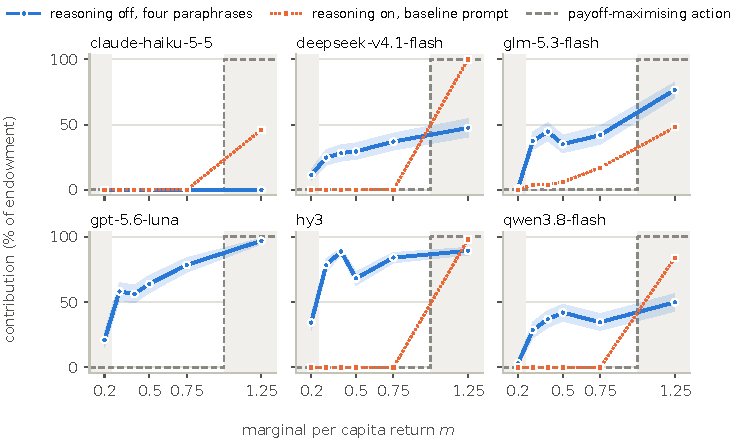
\includegraphics[width=0.8\textwidth]{figures/fig_incentive_response_curves.pdf}
\caption{Study 1. Mean contribution against the marginal per capita return, with reasoning off (blue, four paraphrases pooled, 95\% intervals) and on (orange, baseline prompt). The dashed line is the payoff-maximising action and shaded areas are the controls.}
\label{fig:curves}
\end{figure}

\begin{table}[t]
\caption{Study 1, reasoning off, paraphrase set. Slope in percentage points per unit of $m$ inside the dilemma, mean contribution (\%) in each control with the H1b verdict (\checkmark~pass, $\times$~fail, ?~inconclusive), correct answers (\%) to the two comprehension questions, and ratio of the variance explained by incentive and by paraphrase. Brackets are 95\% intervals. $^{*}$Holm-corrected $p<0.05$.}
\label{tab:main}
\centering
\scriptsize
\setlength{\tabcolsep}{4.5pt}
\begin{tabular}{@{}l r@{\ }l c c r r l@{}}
\toprule
 & \multicolumn{2}{c}{Slope (H1a)} & \multicolumn{2}{c}{Controls (H1b)} & \multicolumn{2}{c}{Comprehension} & Signal-to-noise \\
\cmidrule(lr){2-3}\cmidrule(lr){4-5}\cmidrule(lr){6-7}
Model & & & $m{=}0.2$ & $m{=}1.25$ & Q1 & Q2 & \\
\midrule
gpt-5.6-luna & $49.7^{*}$ & [33.2, 65.8] & 21.0 $\times$ & 97.0 \checkmark & 86 & 0 & 0.18 [0.09, 0.34] \\
deepseek-v4.1-flash & $26.6^{*}$ & [8.8, 44.1] & 11.3 ? & 47.5 $\times$ & 83 & 40 & 0.07 [0.01, 0.22] \\
qwen3.8-flash & 9.1 & [$-$7.2, 26.0] & 3.0 \checkmark & 49.9 $\times$ & 88 & 7 & 0.06 [0.02, 0.19] \\
glm-5.3-flash & 4.6 & [$-$12.4, 21.4] & 1.0 \checkmark & 76.6 $\times$ & 82 & 3 & 0.05 [0.01, 0.19] \\
hy3 & 4.2 & [$-$7.5, 16.1] & 34.4 $\times$ & 89.3 ? & 88 & 18 & 0.33 [0.22, 0.48] \\
claude-haiku-5-5 & 0.0 & [0.0, 0.0] & 0.0 \checkmark & 0.0 $\times$ & 100 & 100 & undefined \\
\bottomrule
\end{tabular}
\end{table}

No model passes both controls (H1b). Where contributing is wasteful, three models contribute almost nothing, one is inconclusive and two fail, with 21\% and 34\%. Where contributing everything is dominant, only \texttt{gpt-5.6-luna} passes, and three models contribute about half or less. In the comprehension questions most models compute the payoff of a full contributor among non-contributors (Q1), but five of six fail the mirror question (Q2). \texttt{claude-haiku-5-5} answers both correctly in every call and still contributes nothing when contributing is dominant.

\subsection{Paraphrase versus framing}

Wording has a significant main effect in the paraphrase layout for the five models with any variation (Holm-corrected $p<0.001$). The incentive explains between 0.6\% and 5.8\% of the variance of contributions, and rewording the same game explains between 12.4\% and 18.7\%. The signal-to-noise ratio lies between 0.05 and 0.33, and every upper bound is below 0.5 (Table~\ref{tab:main}), so paraphrase accounts for 3 to 21 times more variance than the incentive. Framing explains more than paraphrase in four of the five models, between 28\% and 67\%. For \texttt{qwen3.8-flash} the two are indistinguishable (difference $-0.01$ [$-0.07$, 0.05]). For \texttt{claude-haiku-5-5} nothing varies in the paraphrase layout, so the ratio is undefined, while framing explains 71\% of its variance. H2 is therefore supported for four of six models.

Table~\ref{tab:variants} gives the means behind these shares. Within a single model the mean contribution across the four paraphrases ranges over 33 to 55 percentage points, except for \texttt{claude-haiku-5-5}. The paraphrases also interact with the controls. At $m=0.2$ the baseline elicits 2\% and 0\% from \texttt{gpt-5.6-luna} and \texttt{hy3}, whereas P2, which states that each participant receives 0.2 per unit placed, elicits 76\% and 99\%.

\begin{table}[t]
\caption{Study 1, reasoning off. Mean contribution (\% of endowment) inside the dilemma by prompt variant, 200 decisions per cell. The last column gives F3 at $m=1.25$ (50 decisions), where the dominant action is 100.}
\label{tab:variants}
\centering
\scriptsize
\setlength{\tabcolsep}{3.2pt}
\begin{tabular}{@{}l rrrr r rrr r@{}}
\toprule
 & \multicolumn{4}{c}{Paraphrases} & Examples & \multicolumn{3}{c}{Framings} & F3 at \\
\cmidrule(lr){2-5}\cmidrule(lr){6-6}\cmidrule(lr){7-9}
Model & P0 & P1 & P2 & P4 & P3 & F1 take & F2 Teamw. & F3 named & $m{=}1.25$ \\
\midrule
gpt-5.6-luna & 39.5 & 50.0 & 76.5 & 91.0 & 38.0 & 7.0 & 77.8 & 0.0 & 0.0 \\
deepseek-v4.1-flash & 10.5 & 44.8 & 15.9 & 48.3 & 80.0 & 59.8 & 33.1 & 2.0 & 2.0 \\
qwen3.8-flash & 37.3 & 62.0 & 7.5 & 35.4 & 64.5 & 48.8 & 78.4 & 30.6 & 27.1 \\
glm-5.3-flash & 28.0 & 55.2 & 18.0 & 58.0 & 70.5 & 63.9 & 88.0 & 21.6 & 28.5 \\
hy3 & 68.1 & 99.5 & 85.3 & 66.8 & 99.6 & 45.7 & 100.0 & 4.2 & 1.0 \\
claude-haiku-5-5 & 0.0 & 0.0 & 0.0 & 0.0 & 0.0 & 94.0 & 65.0 & 0.0 & 0.0 \\
\bottomrule
\end{tabular}
\end{table}

The framings behave as in earlier reports for the ``Teamwork'' label, which raises contributions in every model. Naming the game does the opposite (H6). Inside the dilemma it lowers contributions significantly for three of the five models that contribute anything at baseline, and four of the six models end at 4.2\% or less. At $m=1.25$, where contributing everything maximises the agent's own payoff, it lowers contributions for all five, by 28 to 90 points, leaving four models at 2\% or less. Their answers match the textbook answer to the named game and not the action implied by the stated payoffs. F3 changes the vocabulary as well as the name, so the two cannot be separated. Under the take frame \texttt{claude-haiku-5-5} answers with the number zero in 96\% of its decisions, as it does in all of them under the baseline, so the same answer counts as full contribution in one description and as none in the other.

\section{Results of Study 2}

\subsection{Reasoning and wording}

{\sloppy Table~\ref{tab:reasoning} repeats the comparison of wordings with reasoning on. Every decision inside the dilemma is zero under all eight variants for \texttt{hy3} and \texttt{deepseek-v4.1-flash}, and under seven for \texttt{qwen3.8-flash}. A1 is supported for four of five models. The paraphrase range falls from between 33 and 55 points to zero in three of them and from 40.0 to 17.8 in \texttt{glm-5.3-flash}. The fifth, \texttt{claude-haiku-5-5}, already contributed nothing under every paraphrase without reasoning. A2 is supported for all five, although the ``Teamwork'' label still raises contributions to 41.2\% in \texttt{glm-5.3-flash} and to 20.8\% in \texttt{qwen3.8-flash}. The baseline cells did not differ from those of Study~1. With reasoning on, the returned text of 90\% to 100\% of decisions under the neutral prompt of Study~1 contains game-theoretic vocabulary such as ``Nash'' or ``free rider'', against less than 1\% with reasoning off. This is a count of words and says nothing about how the action was produced.\par}

Reasoning therefore removes paraphrase sensitivity inside the dilemma mostly by putting contributions at the floor. Where the floor does not bind, the sensitivity is still there. At $m=1.25$, where contributing everything is dominant, \texttt{deepseek-v4.1-flash} and \texttt{hy3} contribute 98\% or more under every variant and pass both controls. \texttt{claude-haiku-5-5} ranges from 16\% to 98\% across variants and \texttt{glm-5.3-flash} from 14\% to 84\%, and both fail that control. Naming the game lowers contributions there from 66\% to 14\% in \texttt{glm-5.3-flash} and from 54\% to 30\% in \texttt{claude-haiku-5-5}.

\begin{table}[t]
\caption{Study 2, reasoning on. Mean contribution (\% of endowment) inside the dilemma by prompt variant, 200 decisions per cell, paraphrase range (points) with reasoning off and on, and lowest and highest variant mean at $m=1.25$.}
\label{tab:reasoning}
\centering
\scriptsize
\setlength{\tabcolsep}{3.2pt}
\begin{tabular}{@{}l rrrr r rrr rr c@{}}
\toprule
 & \multicolumn{4}{c}{Paraphrases} & Ex. & \multicolumn{3}{c}{Framings} & \multicolumn{2}{c}{Range} & $m{=}1.25$ \\
\cmidrule(lr){2-5}\cmidrule(lr){6-6}\cmidrule(lr){7-9}\cmidrule(lr){10-11}
Model & P0 & P1 & P2 & P4 & P3 & F1 & F2 & F3 & off & on & min--max \\
\midrule
deepseek-v4.1-flash & 0 & 0 & 0 & 0 & 0 & 0 & 0 & 0 & 37.8 & 0 & 98--100 \\
hy3 & 0 & 0 & 0 & 0 & 0 & 0 & 0 & 0 & 32.7 & 0 & 98--100 \\
qwen3.8-flash & 0 & 0 & 0 & 0 & 0 & 0 & 20.8 & 0 & 54.5 & 0 & 90--98 \\
claude-haiku-5-5 & 0 & 0.5 & 0 & 0 & 0 & 1.0 & 4.0 & 0 & 0 & 0.5 & 16--98 \\
glm-5.3-flash & 8.0 & 6.8 & 24.5 & 10.5 & 29.0 & 15.1 & 41.2 & 6.0 & 40.0 & 17.8 & 14--84 \\
\bottomrule
\end{tabular}
\end{table}

\subsection{Repeated game}

Figure~\ref{fig:traj} shows the ten-round games with reasoning off. D1 is supported for three of six models. In round 10 the gap between the ``Teamwork'' label and the named game is 86.7 points for \texttt{hy3}, 56.8 for \texttt{qwen3.8-flash} and 31.6 for \texttt{glm-5.3-flash}, with adjusted intervals above zero. For the other three the adjusted interval excludes gaps of 20 points. \texttt{gpt-5.6-luna} starts with a gap of 46.7 points that has gone by round 10 (0.7), because contributions under the label fall from 71.7\% to 11.3\%. The wording effect persists where contributions stay high and disappears where they decay.

\begin{figure}[t]
\centering
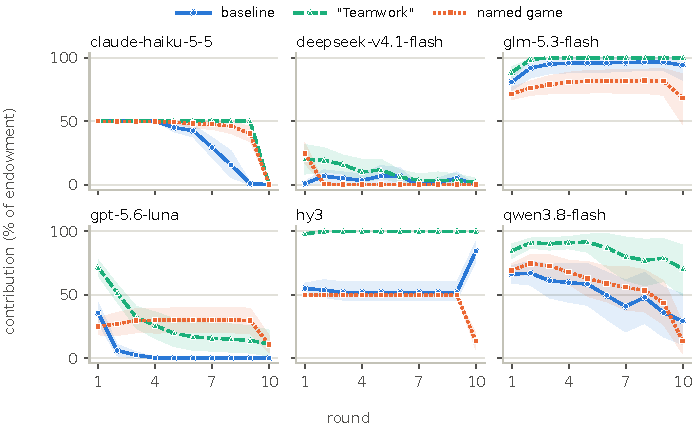
\includegraphics[width=0.8\textwidth]{figures/fig_repeated_trajectories.pdf}
\caption{Repeated game, reasoning off. Mean contribution by round in groups of four agents of the same model, 15 groups per line, with 95\% intervals over groups.}
\label{fig:traj}
\end{figure}

The decline that characterises human groups (D2) appears under the baseline wording in three models, with slopes of $-6.3$, $-4.1$ and $-2.3$ points per round for \texttt{claude-haiku-5-5}, \texttt{qwen3.8-flash} and \texttt{gpt-5.6-luna}. Contributions rise in \texttt{glm-5.3-flash} and \texttt{hy3}, and \texttt{deepseek-v4.1-flash} stays near zero. The response to the others' previous mean (D3) is positive in four models and substantial only in \texttt{claude-haiku-5-5} (0.56 [0.46, 0.65]) and \texttt{qwen3.8-flash} (0.22 [0.01, 0.45]). Some trajectories have no human counterpart. \texttt{claude-haiku-5-5}, which contributed nothing in the one-shot game, contributes exactly half in round 1 under every wording, and under the ``Teamwork'' label all of its agents contribute half for nine rounds and then zero.

With one agent that never contributes in the group, the LLM agents contribute 20 to 34 points less in rounds 2 to 10 in three models. In the exploratory arm with reasoning, \texttt{glm-5.3-flash} falls from between 59\% and 79\% to between 2\% and 33\% by round 10, whereas without reasoning it rises to 94\% or more under two wordings.

\paragraph{Stability between batches.} The round-1 prompt under the baseline wording is the same text in the homogeneous groups and in the groups with a rule-based agent, and the two sets were collected in separate batches. Five models differ by at most 5.3 points between them. \texttt{hy3} answered with the full endowment in 91\% of 45 decisions in the first batch and in 10\% of 60 decisions in the second, which began 22 minutes after the first ended. Nothing in our requests changed, and the comparison with the rule-based agent is uninformative for that model.

\section{Discussion}

\paragraph{Which reference do the agents resemble?} The answer depends on whether reasoning is switched on. With reasoning, most of the models tested behave as the players of the Nash prediction, which is also the prediction of the \emph{Wealth of Nations} for public works. They contribute nothing inside the dilemma under any wording, and two of five choose the dominant action in both controls. This extends earlier findings that reasoning lowers cooperation~\cite{li2025spontaneous,kitadai2025reasoning} to a continuous action, a sweep of the return and eight wordings. Without reasoning the same models resemble none of the references. Their average contribution can be made to look like the generosity of the \emph{Moral Sentiments}, like laboratory subjects, or like free riders by changing words that leave the payoffs untouched, and only two of six respond to the return in the way people do. Interaction does not repair this, since in half of the models a label still separates contributions after ten rounds of feedback.

\paragraph{Implications for modellers.} First, the reasoning mode and the wording are parameters of the model and should be reported and varied like any other. Second, a paraphrase audit is cheap, about 800 calls per model here, and shows whether the simulated behaviour reflects the mechanism or the phrasing. Third, a stable outcome is not evidence of an applied rule. Reasoning made three models insensitive to wording by fixing their answer at zero, and conditions in which every disposition implies the same action were needed to separate the two models that apply the payoff rule from those that do not. Fourth, naming a well-known scenario can elicit its textbook answer even where it contradicts the stated payoffs, which is consistent with the concern about data leakage~\cite{larooij2026validation}, although our design does not identify the cause. Fifth, a hosted model can change its answers to an identical request within the hour, so replications should be collected in interleaved batches and dated.

\paragraph{Limitations.} The audit covers six models of the fast, low-cost tier, accessed through an intermediary over two days. The served versions are those reported by the provider, and frontier models were not tested. It covers one group size, one endowment, English prompts and one temperature, and the repeated game uses one return. Study~2 compares reasoning on with reasoning-off data collected a day earlier. Its plan was public before the run but was not posted to a registry, and that of Study~1 was not public beforehand. We did not study communication, networks or mixed populations of models.

\section{Conclusion}

Used without explicit reasoning, five of six current fast-tier LLMs responded more to how a public goods game was worded than to its payoffs, and none of the six chose the dominant action in both control conditions. With reasoning, most contributed nothing under any wording, and two applied the payoff rule where it prescribes contributing. Repeated interaction preserved the effect of a label in half of the models. An LLM decision rule should therefore be audited against payoff-equivalent rewordings, out-of-dilemma controls and repeated batches before its collective outcomes are interpreted.

\begin{credits}
\subsubsection{Data and code availability.} Code, prompts, configurations, the full ODD description, the preregistration and all raw responses are available at \url{https://github.com/Pepebeats-flp/llm-public-goods-audit}.

\subsubsection{Use of AI tools.} An AI coding assistant (Claude, Anthropic) was used to write the code, run the analysis, and draft and revise the text. The authors take full responsibility for the content.

\subsubsection{\discintname}
The authors have no competing interests to declare that are relevant to the content of this article.
\end{credits}

\bibliographystyle{splncs04}
\bibliography{references}

\end{document}
